%%%%%%%%%%%%%%%%%%%%%%%%%%%%%%%%%%%%%%%%%%%%%%%%%%%%%%%%%%%%%%%

% Set up document

\documentclass{beamer}
\usecolortheme{whale}
\setbeamersize{text margin left=5mm,text margin right=5mm}

% Used to create a section slide between section
\AtBeginSection[]{
  \begin{frame}
  \vfill
  \centering
  \begin{beamercolorbox}[sep=8pt,center,shadow=true,rounded=true]{title}
    \usebeamerfont{title}\insertsectionhead\par%
  \end{beamercolorbox}
  \vfill
  \end{frame}
}

% Remove default navigation symbols and add just  page number
\setbeamertemplate{navigation symbols}{} % Clear default navigation
\addtobeamertemplate{navigation symbols}{}{%
    \usebeamerfont{footline}%
    \usebeamercolor[fg]{footline}%
    \hspace{1em}%
    \insertframenumber/\inserttotalframenumber
}

% CC licence
\usepackage[
    type={CC},
    modifier={by-nc-sa},
    version={3.0},
]{doclicense}


\usepackage{url}
%%%%%%%%%%%%%%%%%%%%%%%%%%%%%%%%%%%%%%%%%%%%%%%%%%%%%%%%%%%%%%%

% Title page

\title{What would other emergency stroke teams do?}
\subtitle{Using explainable machine learning to understand variation in thrombolysis practice}


\author{Kerry Pearn\inst{1}, Michael Allen\inst{1,3}, Anna Laws\inst{1}, Richard Everson\inst{3}, Martin James\inst{1,2} }
\institute{\inst{1}University of Exeter Medical School \inst{2}Royal Devon University Healthcare NHS Foundation Trust \inst{3}University of Exeter Institute of Data Science and Artificial Intelligence}

%\institute{Overleaf}
%\date{March 2023}


\begin{document}

%\frame{\titlepage}

\begin{frame}
\titlepage

\end{frame}

\section{General findings}

\begin{frame}
\frametitle{Thrombolysis rates vary .... a lot}
Here is the range of thrombolysis use across the 132 acute stroke centres in England and Wales, 2016-2018.
\begin{center}
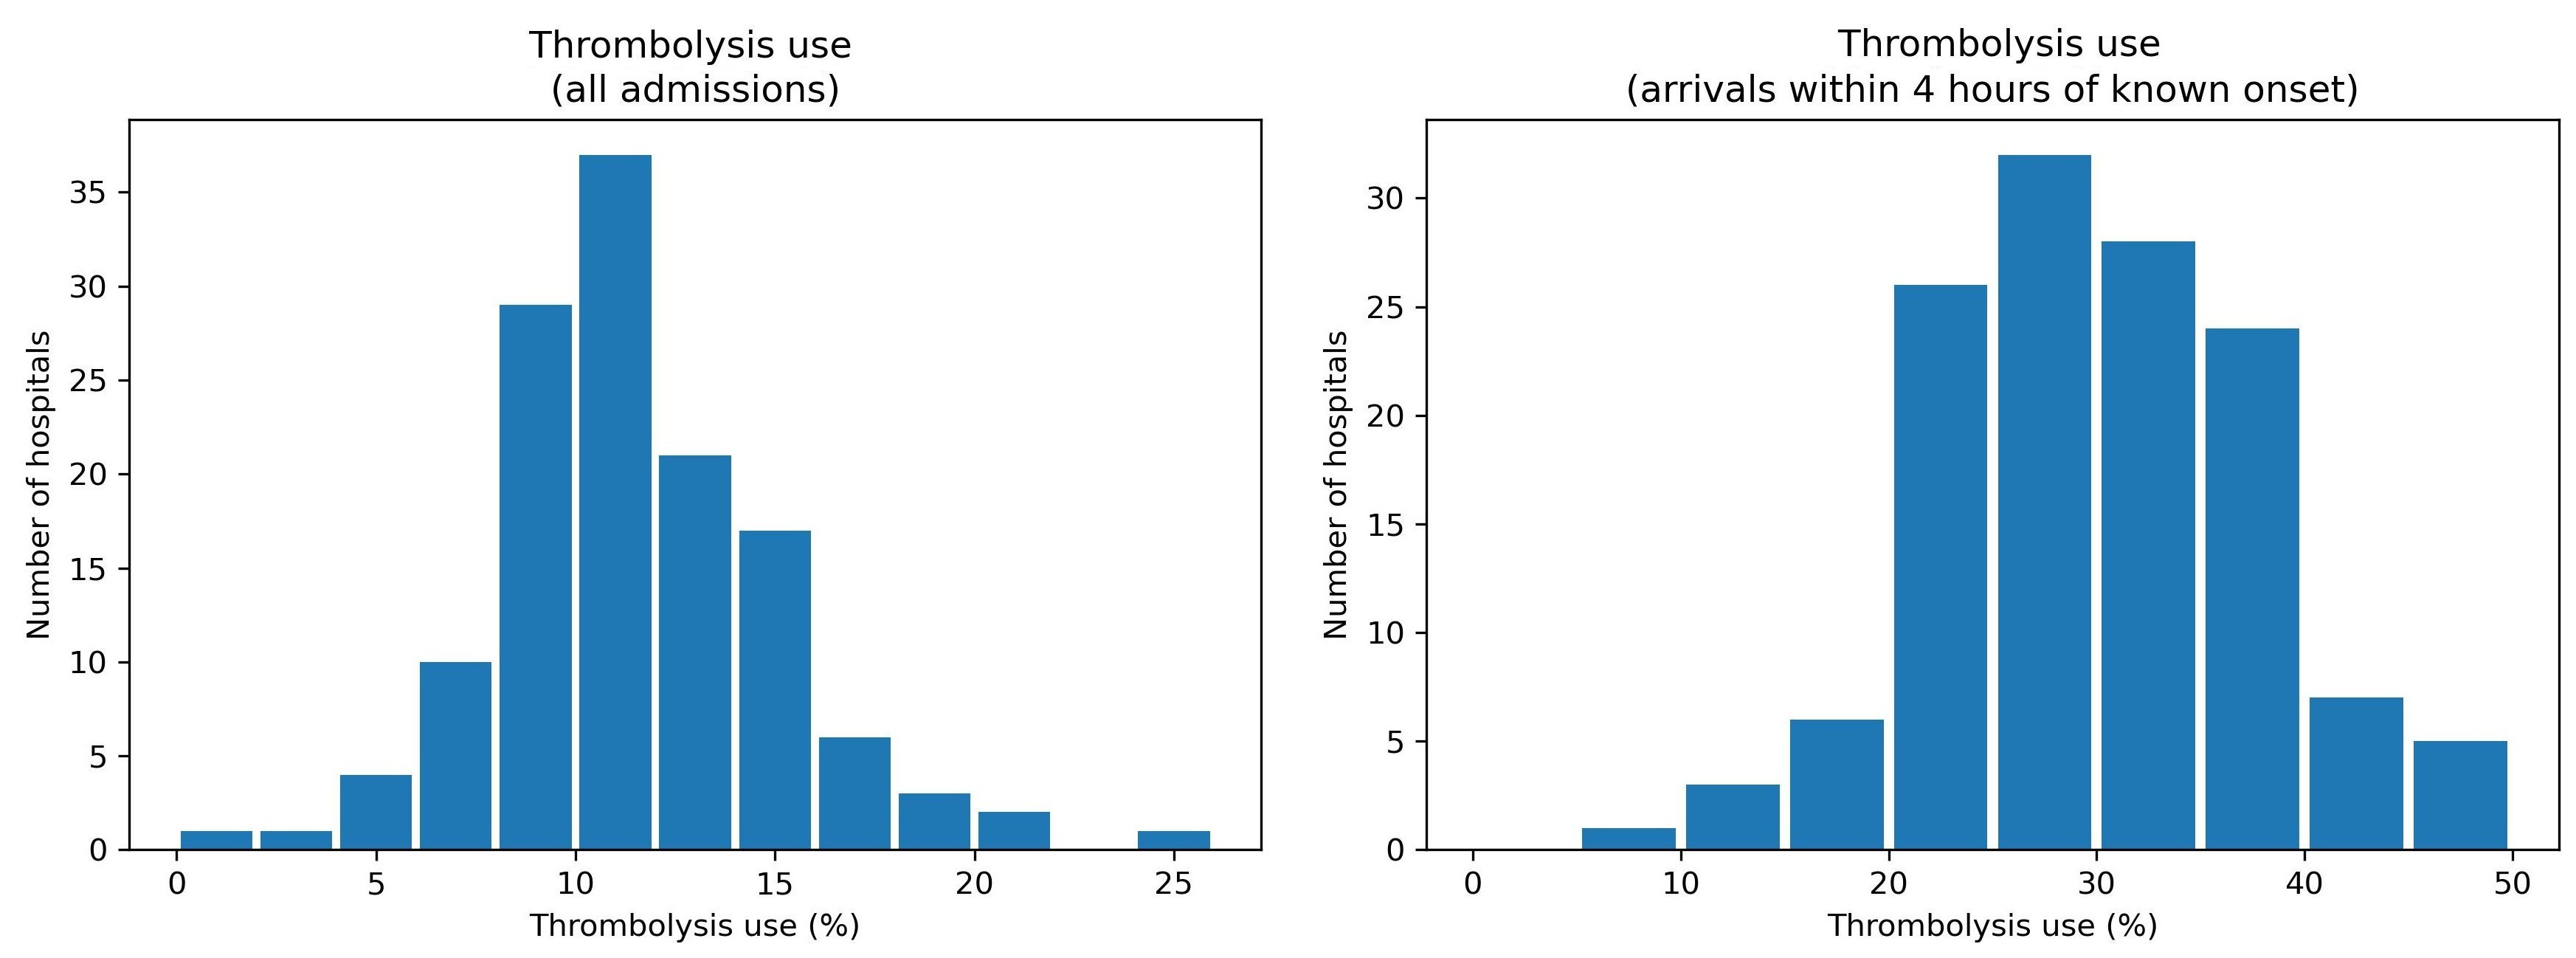
\includegraphics[width=1.0\textwidth]{./images/thrombolysis_hist}
\end{center}

How much of this variation is due to differences in local patient populations, and how much is due to differences in decisions hospitals make on who they would give thrombolysis to?
\end{frame}
\begin{frame}
\frametitle{Breaking down the emergency stroke pathway into key steps}
\begin{center}
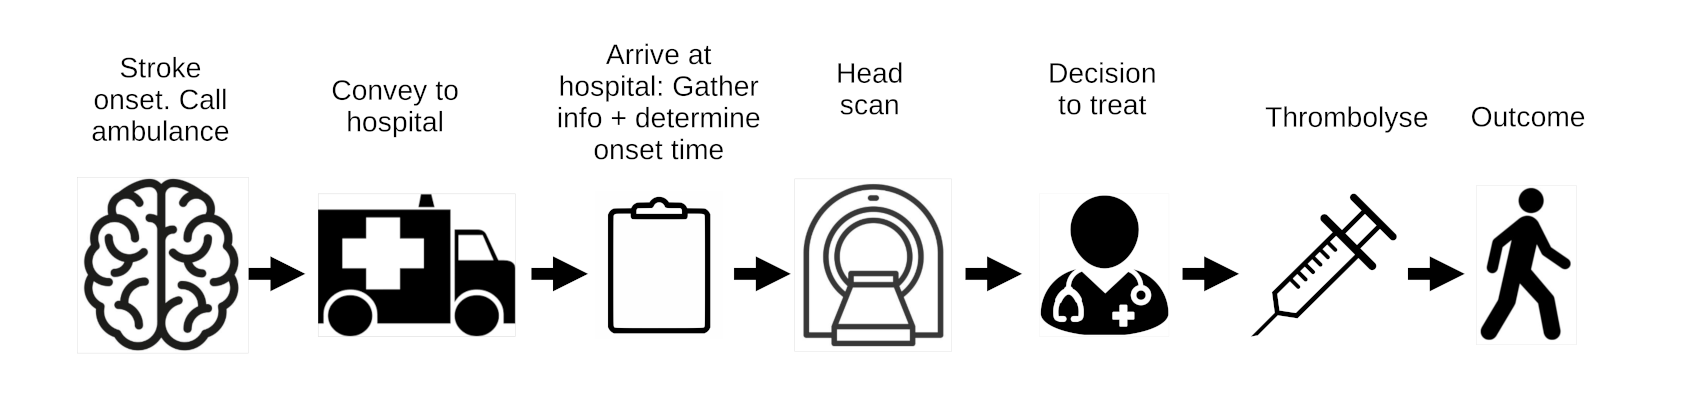
\includegraphics[width=1.0\textwidth]{./images/pathway}
\end{center}
We can model key changes to pathway, such as:
\begin{small}
\begin{itemize}
    \item What if the pathway were \textbf{faster}?
    \item What if hospital \textbf{determined the stroke onset time} in more patients?
    \item What if clinical \textbf{decision-making} was like that of \emph{benchmark} hospitals? (Predict what treatment a patient would receive at other hospitals).
\end{itemize}
\end{small}
\footnotesize{We model these changes with a hospital's own patient population, to allow for inter-hospital variation in patient population characteristics.}
\end{frame}
\begin{frame}
\frametitle{Our Approach}

\small

\begin{itemize}
    \item Train a machine learning algorithm to learn to predict to which patients each hospital would, or would not, give thrombolysis.
    \item Identify the patient characteristics which are most important in predicting use of thrombolysis, and produce a simpler machine learning model based on these characteristics.
    \item Identify \emph{ideal} candidates for thrombolysis.
    \item Add an \emph{explainable machine learning} layer* to understand patterns of use of thrombolysis.
    \item Investigate what we think would happen if every hospital received exactly the same 10k cohort of patients.
    \item Identify key subgroups of patients where hospitals differ in their use of thrombolysis.
\end{itemize}

\vspace{3mm}
\footnotesize
*SHAP (Shapley Additive Values, which provide information on what contribution each patient characteristic makes to the final prediction of whether they will, or will not, receive thrombolysis).
\end{frame}
\begin{frame}
\frametitle{Machine learning overview}
\begin{center}
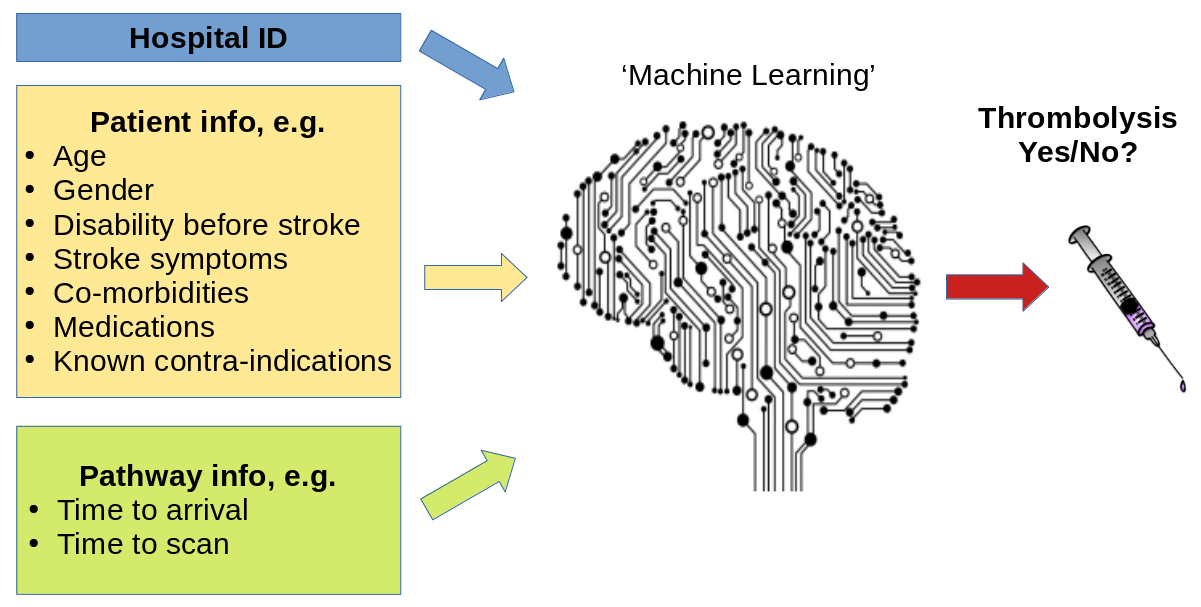
\includegraphics[width=0.80\textwidth]{./images/ml_model_high_level}
\end{center}

\small
\textbf{Machine learning is based on the simple principle of recognising similarity to what has been seen before.}
\vspace{2mm}

\footnotesize{We accessed 246,676 emergency stroke admissions in England and Wales over three years. Our machine learning models use XGBoost classification, and are based on those 88,928 patients who arrive within 4 hours of known stroke onset. Accuracy = 85\% (ROC AUC = 0.92).}
\end{frame}
\begin{frame}
\frametitle{Simplifying our model}

In order to simplify the model, to make it easier to explain, we reduced the number of patient features from 60 to 10, with almost no loss of model accuracy.

\small
\begin{itemize}
    \item \emph{Arrival-to-scan time}: Time from arrival at hospital to scan (mins)
    \item \emph{Infarction}: Stroke type (infarction or haemorrhage)
    \item \emph{Stroke severity}: Stroke severity (NIHSS) on arrival (ranges from 0 to 42)
    \item \emph{Precise onset time}: Onset time is known precisely
    \item \emph{Prior disability level}: Disability level (modified Rankin Scale) before stroke
    \item \emph{Stroke team}: Stroke team attended
    \item \emph{Use of AF anticoagulants}: Use of atrial fibrillation anticoagulant
    \item \emph{Onset-to-arrival time}: Time from onset of stroke to arrival at hospital
    \item \emph{Onset during sleep}: Did stroke occur in sleep?
    \item \emph{Age}: Age (as middle of 5 year age bands)
\end{itemize}
\end{frame}
\begin{frame}{Model accuracy, and simplification}

A model with all available 84 features had an ROC AUC of 0.922. A model with 10 features had an ROC AUC of 0.919.

\begin{center}
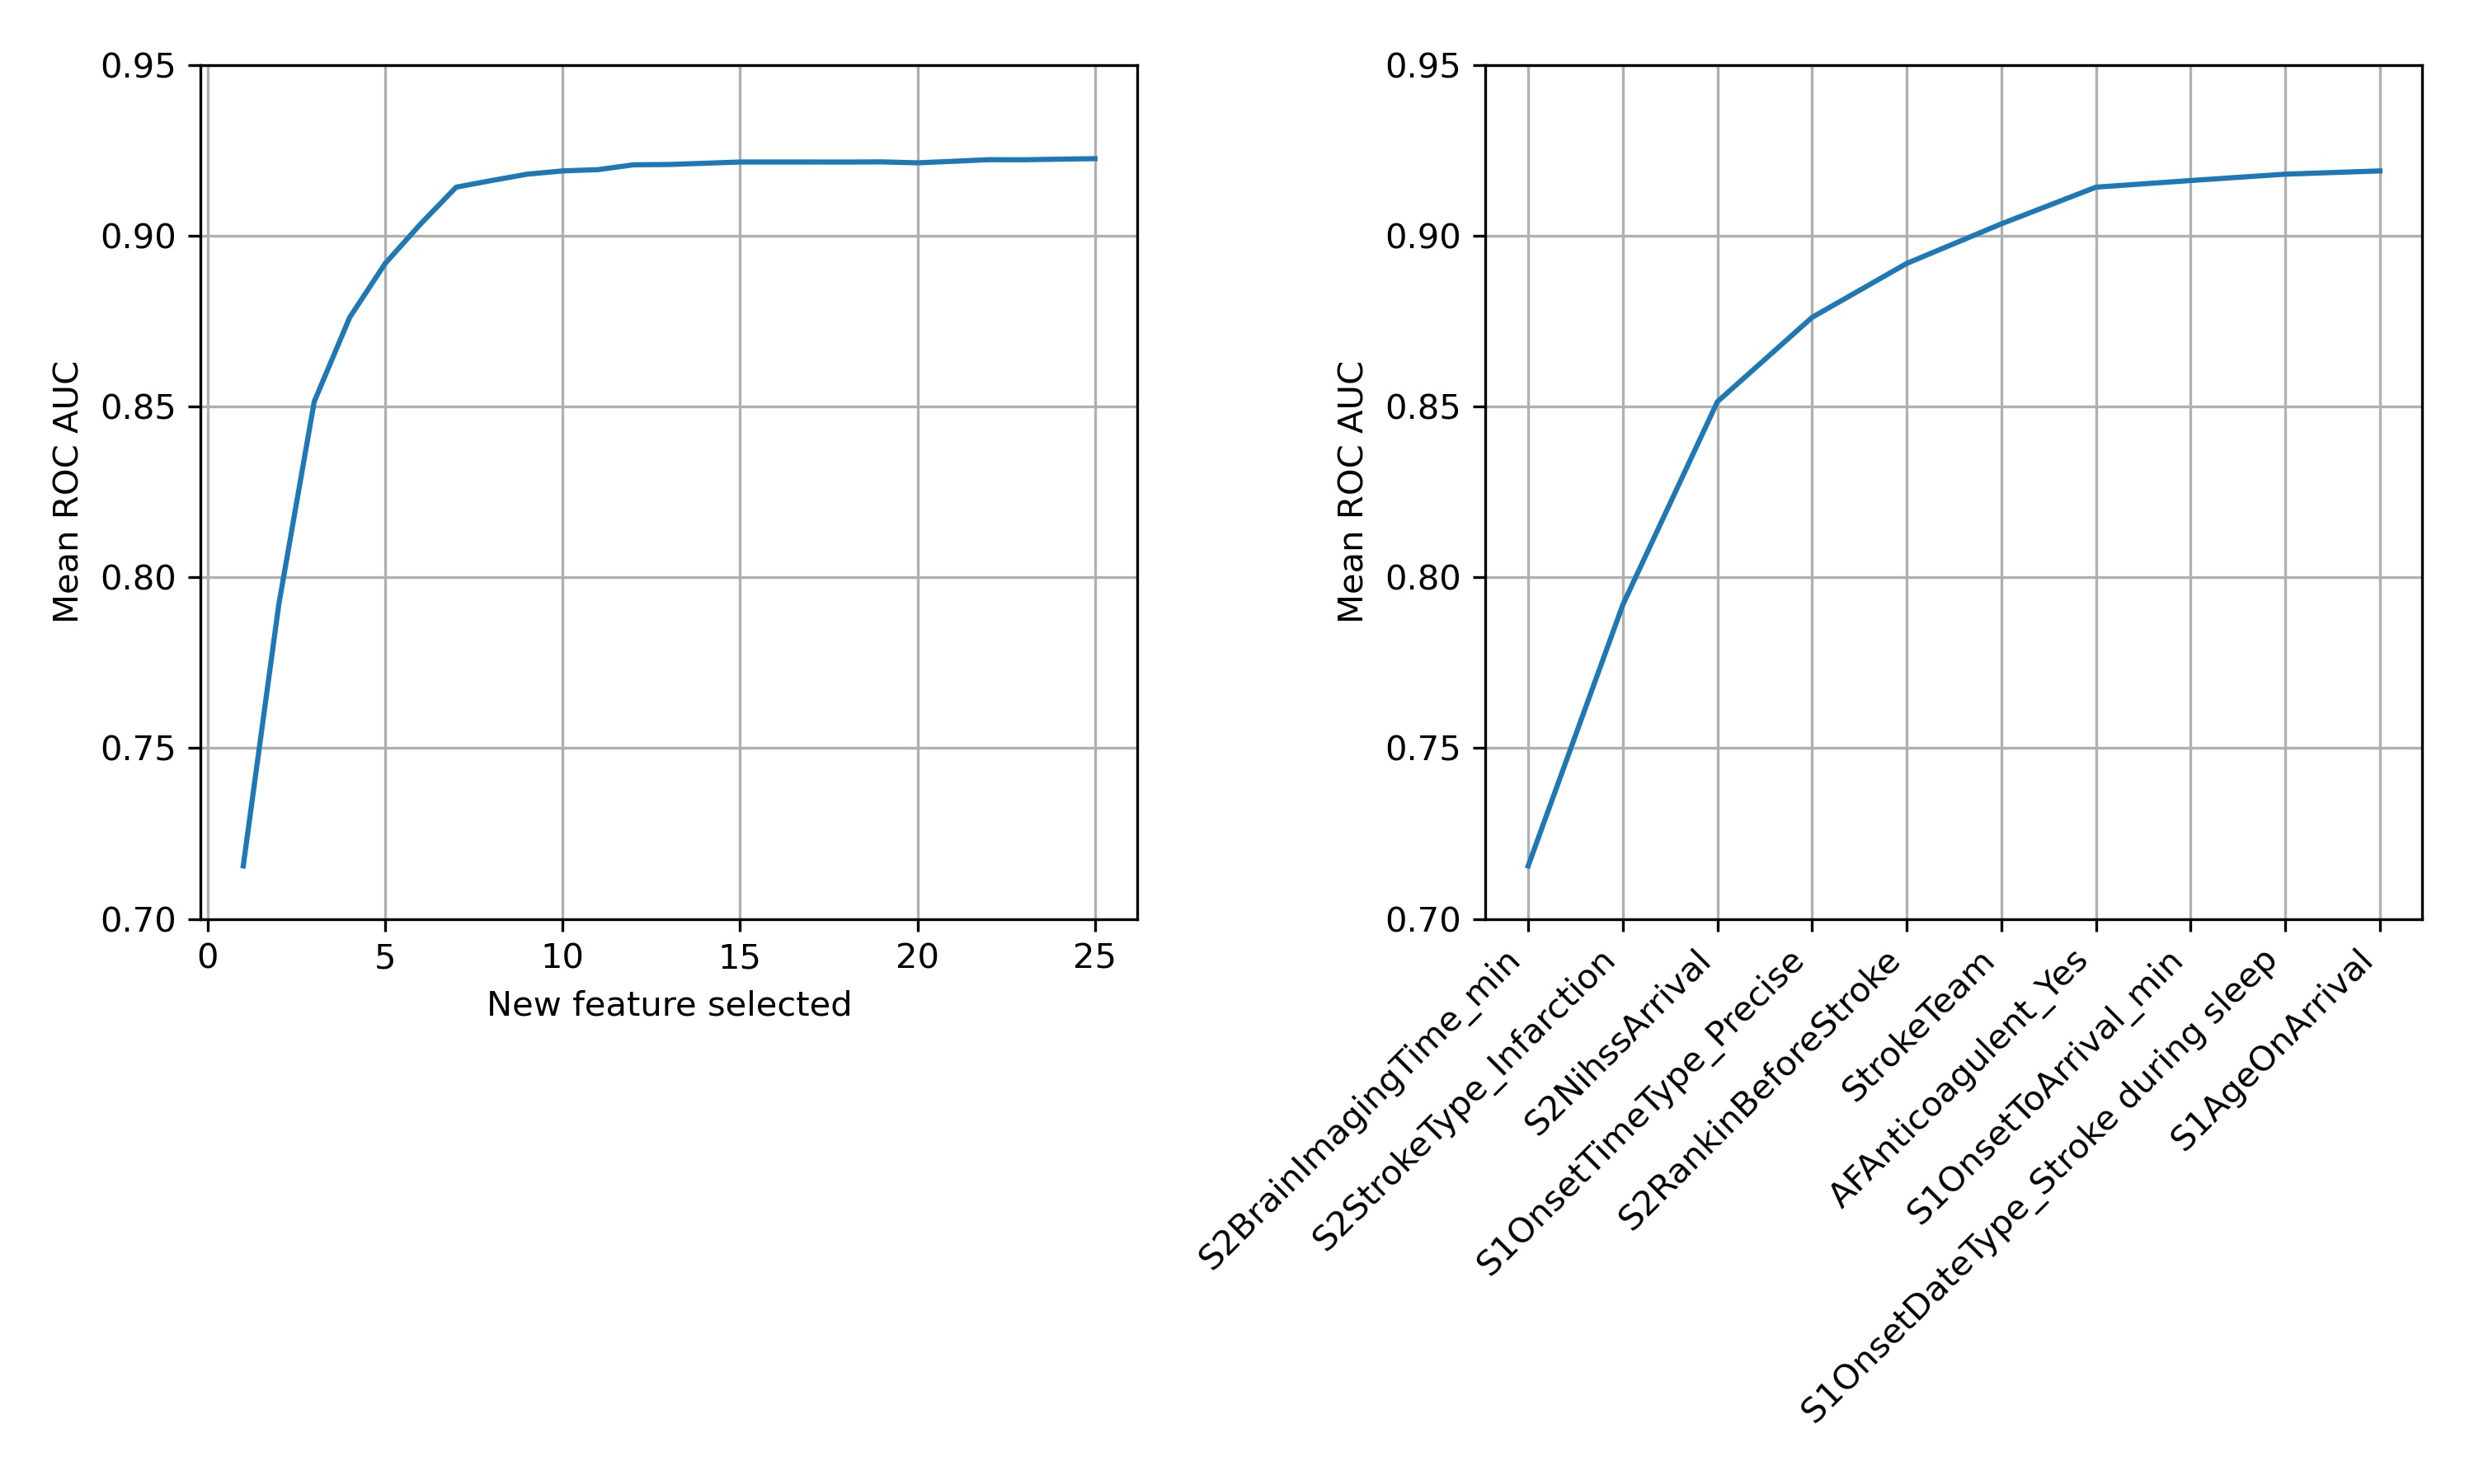
\includegraphics[width=0.9\textwidth]{./images/01_feature_selection.jpg}
\end{center}

Our simpler machine learning model will just use these 10 features.

\end{frame}
\begin{frame}{Predicting hospital thrombolysis use}

Predicted thrombolysis use was measured by combining 5 test sets from k-fold validation. The predicted vs. observed thrombolysis are highly correlated (r-squared 0.977). 

\begin{center}
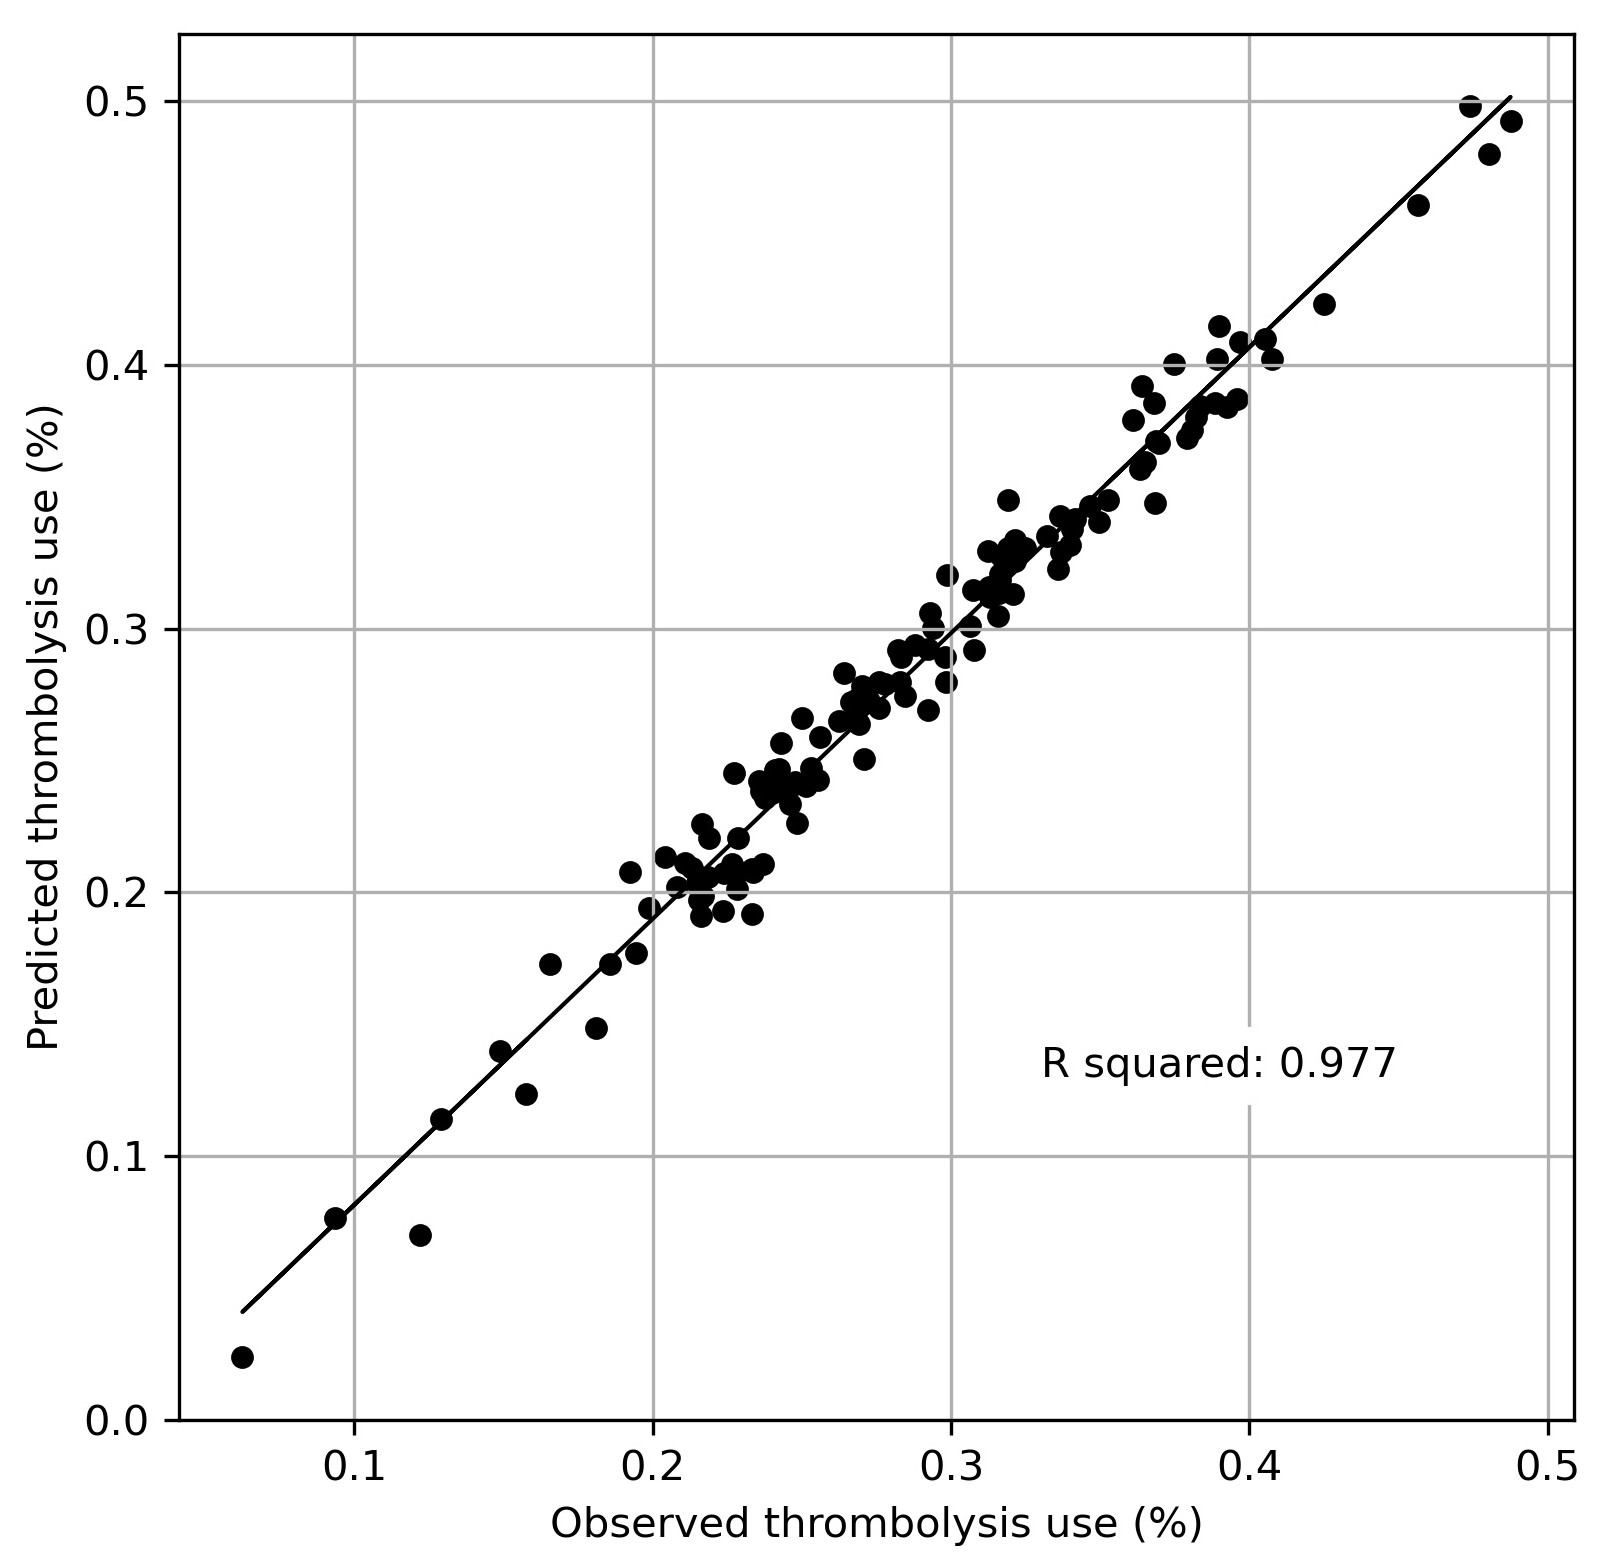
\includegraphics[width=0.55\textwidth]{./images/02_xgb_10_features_observed_predicted_rates.jpg}
\end{center}



\end{frame}
\begin{frame}
\frametitle{Explaining model predictions with SHAP values}

SHAP values show the influence of features (even for \emph{`black box'} models).

\begin{center}
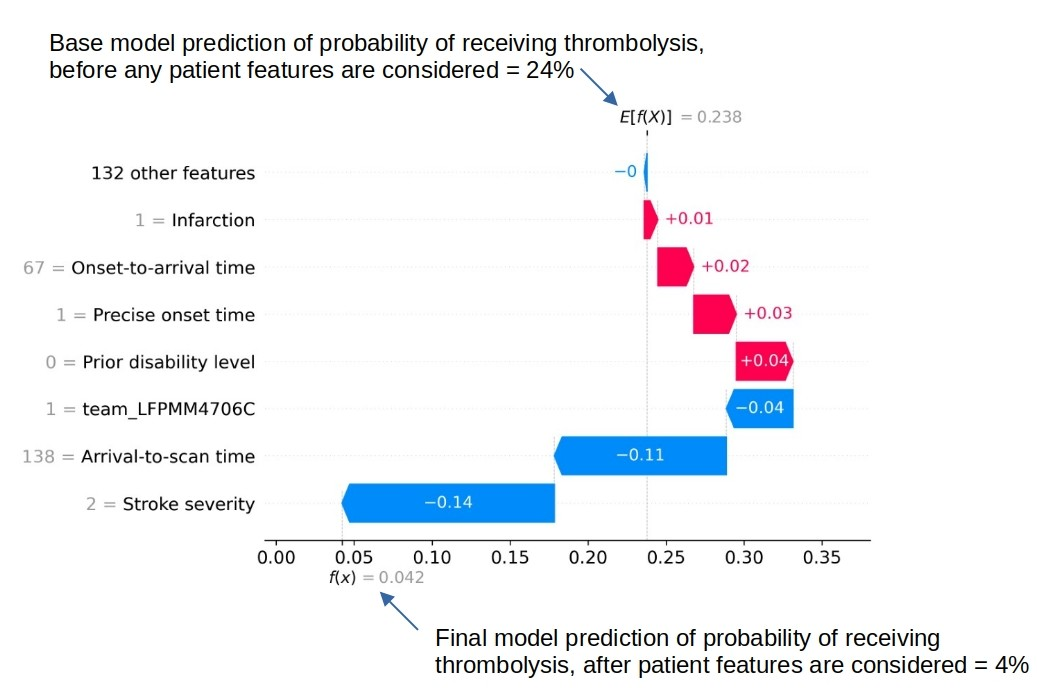
\includegraphics[width=0.90\textwidth]{./images/xgb_waterfall_low_probability_2.jpg}
\end{center}
\end{frame}
\begin{frame}
\frametitle{SHAP values for thrombolysis prediction}
Note: SHAP values here are log odds. 
\begin{center}
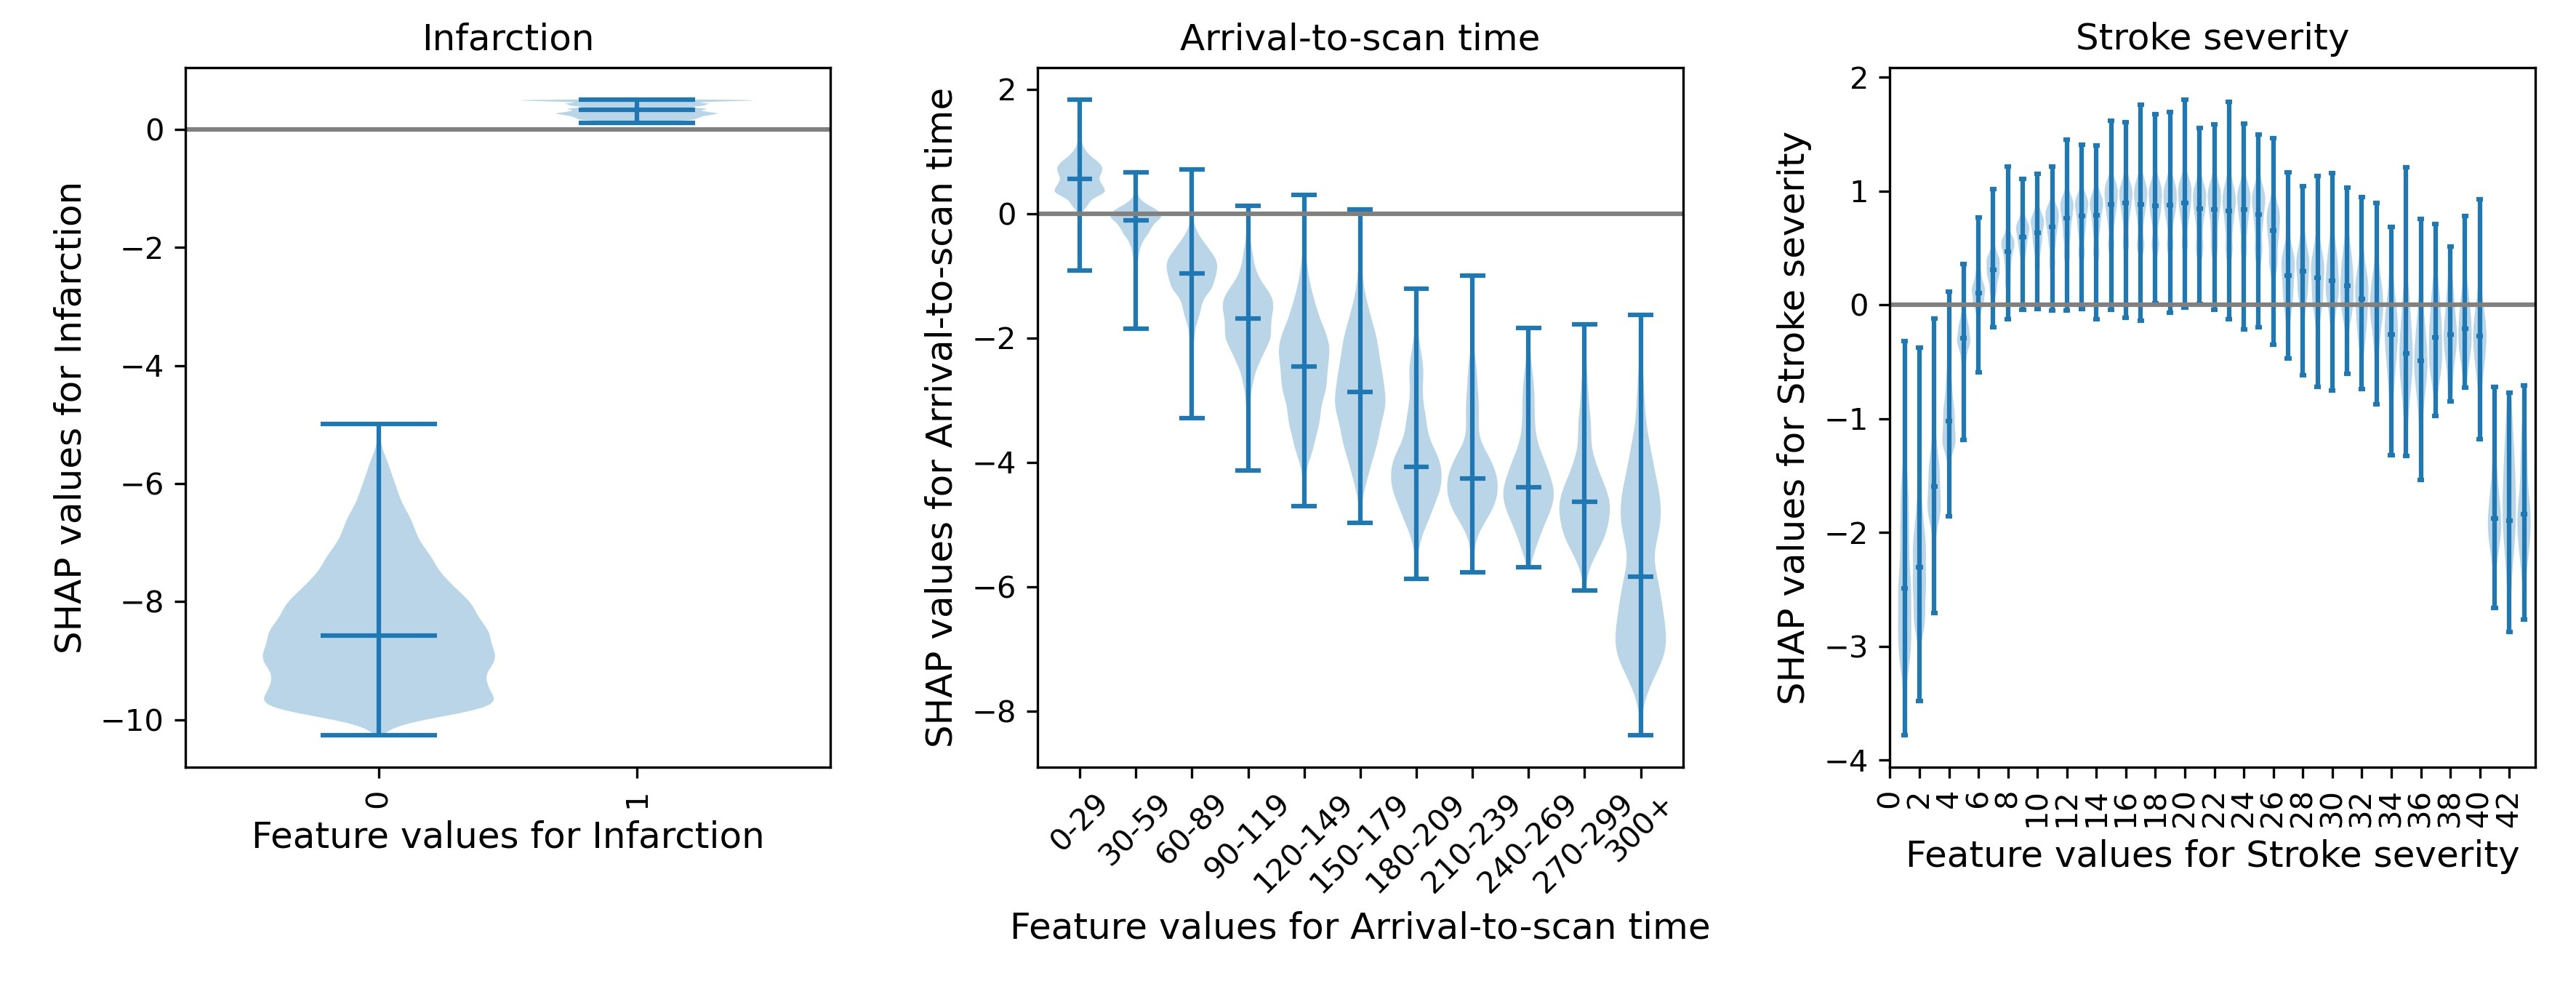
\includegraphics[width=1.0\textwidth]{./images/03d_xgb_10_features_thrombolysis_shap_violin_1.jpg}
\end{center}

\scriptsize
SHAP effects: \\
$\pm1$: Odds change $\pm3$ fold\\
$\pm2$: Odds change $\pm7$ fold\\
$\pm3$: Odds change $\pm20$ fold\\
$\pm4$: Odds change $\pm55$ fold\\
$\pm5$: Odds change $\pm150$ fold
\end{frame}
\begin{frame}
\frametitle{SHAP values for each feature - 2}
Note: SHAP values here are log odds. 
\begin{center}
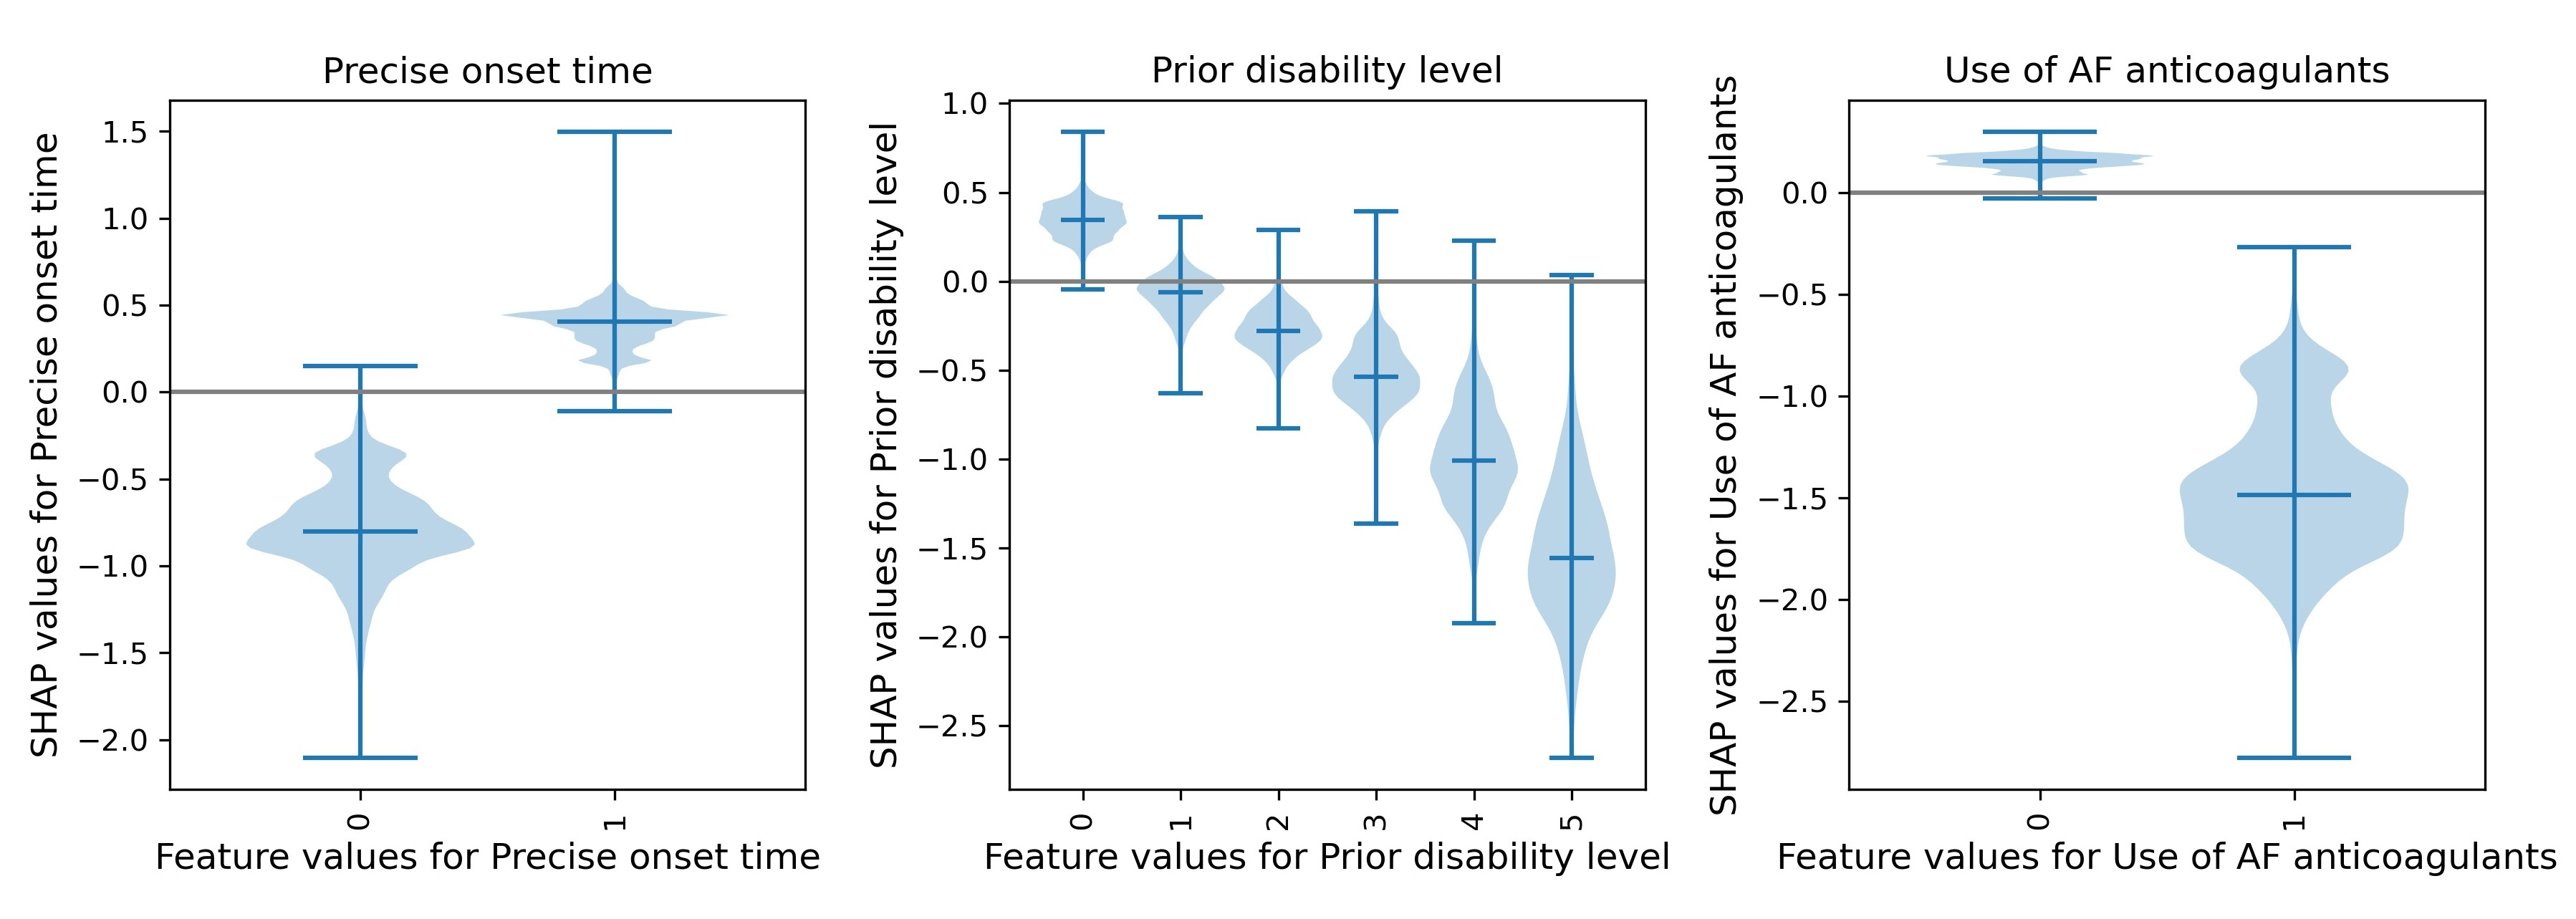
\includegraphics[width=1.0\textwidth]{./images/03d_xgb_10_features_thrombolysis_shap_violin_2.jpg}
\end{center}
\scriptsize
SHAP effects: \\
$\pm1$: Odds change $\pm3$ fold\\
$\pm2$: Odds change $\pm7$ fold\\
$\pm3$: Odds change $\pm20$ fold\\
$\pm4$: Odds change $\pm55$ fold\\
$\pm5$: Odds change $\pm150$ fold
\end{frame}
\begin{frame}
\frametitle{SHAP values for each feature - 3}
Note: SHAP values here are log odds. 
\begin{center}
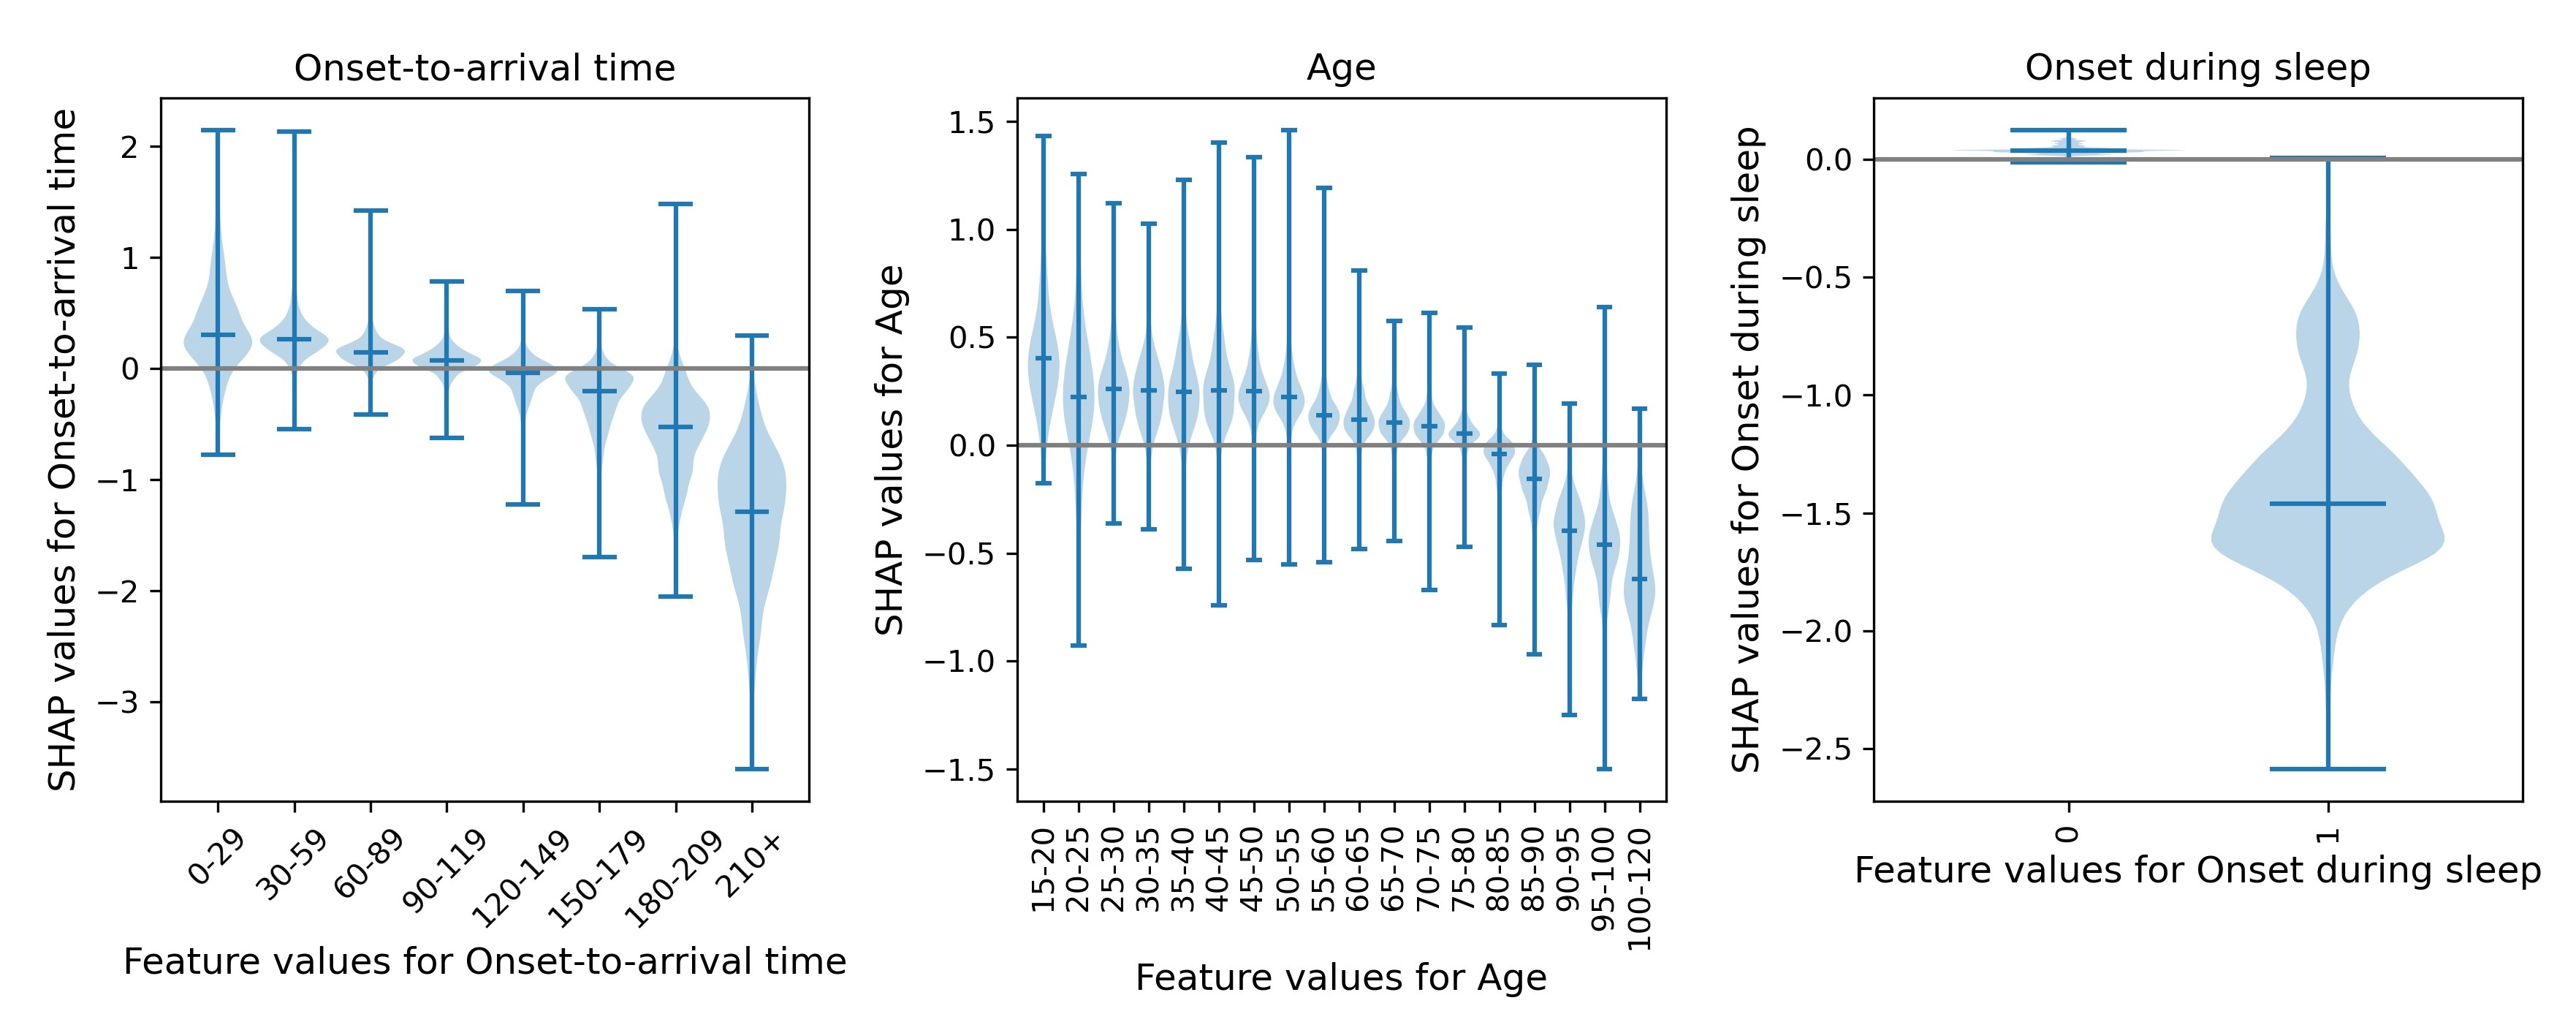
\includegraphics[width=1.0\textwidth]{./images/03d_xgb_10_features_thrombolysis_shap_violin_3.jpg}
\end{center}
\scriptsize
SHAP effects: \\
$\pm1$: Odds change $\pm3$ fold\\
$\pm2$: Odds change $\pm7$ fold\\
$\pm3$: Odds change $\pm20$ fold\\
$\pm4$: Odds change $\pm55$ fold\\
$\pm5$: Odds change $\pm150$ fold
\end{frame}
\begin{frame}
\frametitle{Isolating the effect of hospitals}
Note: SHAP values here are log odds. 
\begin{center}
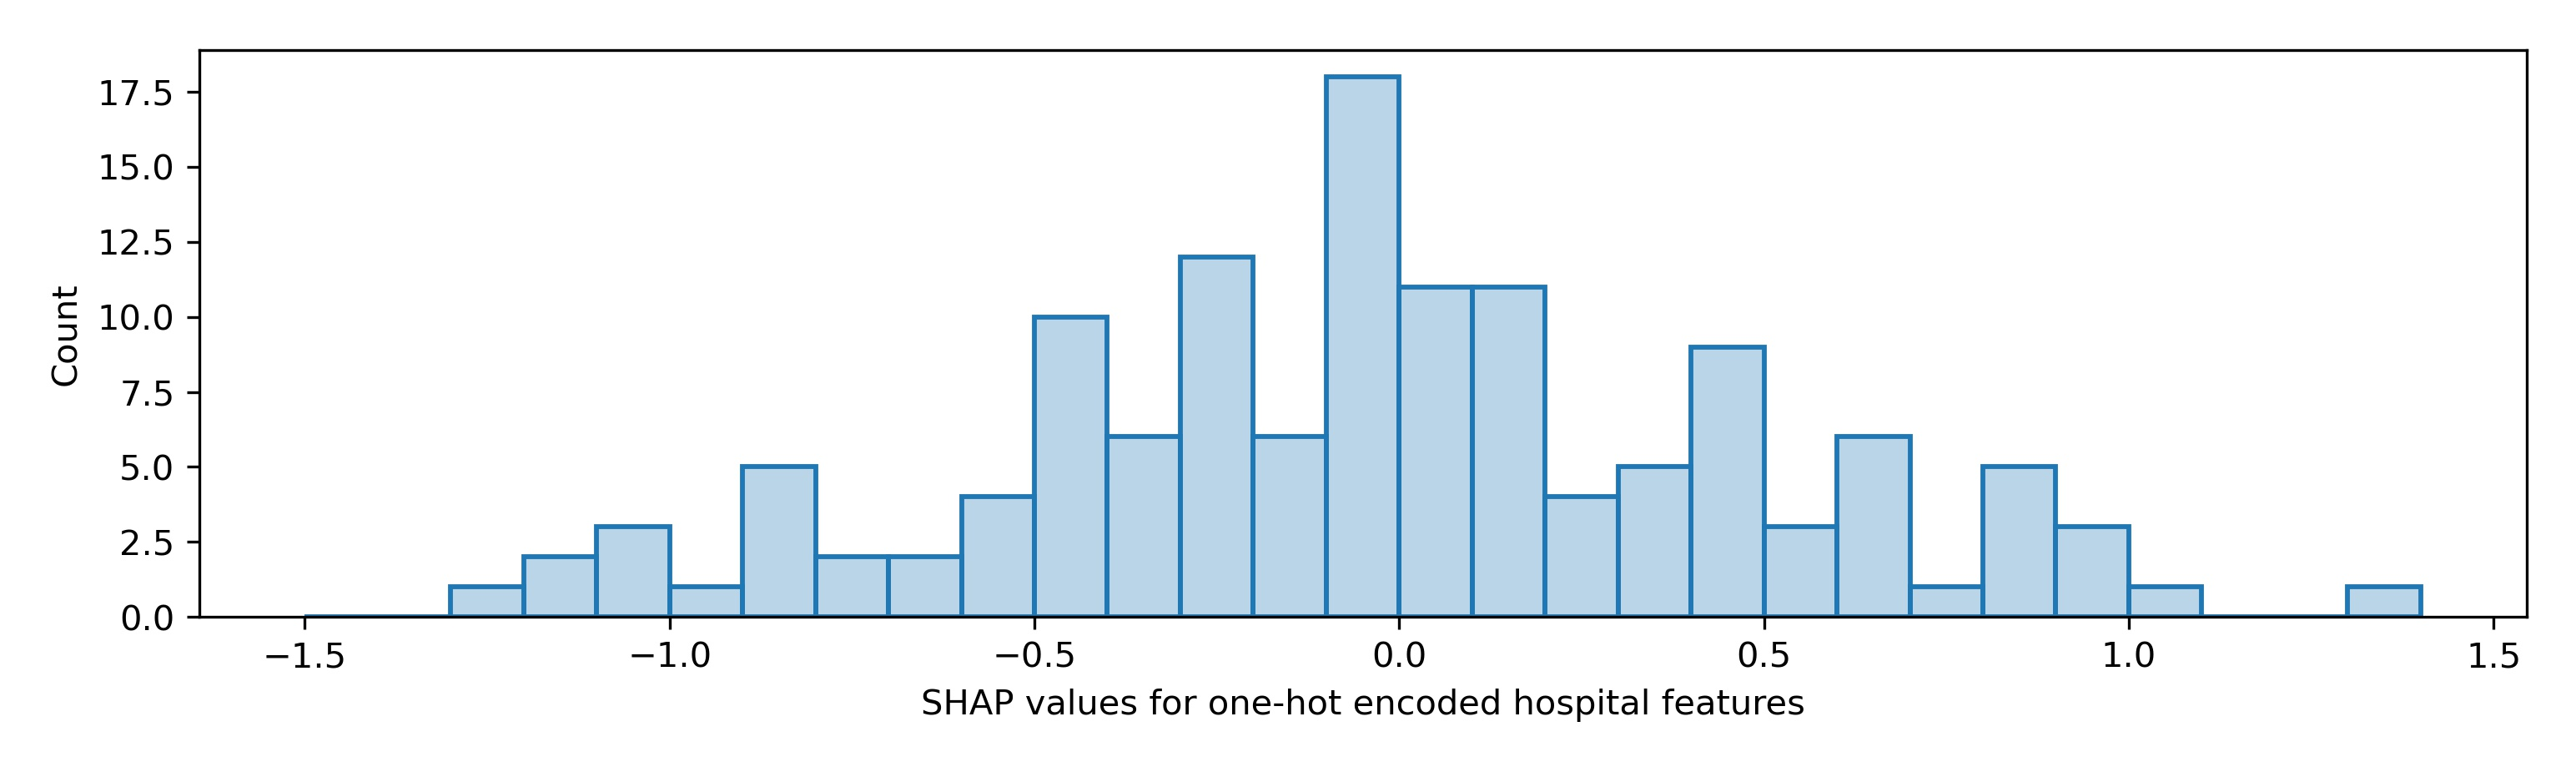
\includegraphics[width=1.0\textwidth]{./images/03d_xgb_10_features_hosp_shap_hist.jpg}
\end{center}
\scriptsize
SHAP effects: \\
$\pm1$: Odds change $\pm3$ fold\\
$\pm2$: Odds change $\pm7$ fold\\
$\pm3$: Odds change $\pm20$ fold\\
$\pm4$: Odds change $\pm55$ fold\\
$\pm5$: Odds change $\pm150$ fold
\end{frame}
\begin{frame}
\frametitle{What drives use of thrombolysis across all hospitals?}

The XGBoost/SHAP model revealed that the odds of receiving thrombolysis:

\vspace{2mm}

\begin{itemize}
    \setlength{\itemsep}{1.5mm}
    \item Reduced 20 fold over the first 100 minutes of arrival-to-scan time.
    \item Varied 30 fold depending on stroke severity.
    \item Reduced 3 fold with imprecise onset time.
    \item Fell 5 fold with increasing pre-stroke disability.
    \item Varied 15 fold between hospitals. 
    \item Fell 5 fold if the patient was taking anticoagulant medication.
    \item Was stable for the first two hours of arrival-to-onset time,and then fell 3 fold between two and four hours arrival-to-onset time
    \item Fell 2 fold between the age of 80 and 110.
    \item Fell 4 fold if onset was during sleep (these patients will also have the reduction due to imprecise onset time). 
\end{itemize}

\end{frame}

\section{Sussex results}

\begin{frame}
\frametitle{Sussex modelling}


The results and modelling presented here are based on 2017-2019 (pre-covid).

\vspace{6mm}

The results observed fit into general patterns seen across England and Wales - no Sussex unit is \emph{unusual}.


\end{frame}

\begin{frame}
\frametitle{Sussex descriptive statistics (4hr arrivals)}

\scriptsize
\begin{table}[]
\begin{tabular}{llllll}
                            & All E+W & Worthing & St Richards & R. Sussex & Eastborn \\
\hline
thrombolysis (all arrivals)	        & 0.138	  & 0.167	 & 0.154	   & 0.106	   & 0.093    \\
onset known (all arrivals)          & 0.707   & 0.698    & 0.957       & 0.494     & 0.620    \\
arrive in 4 hours (all arrivals)    & 0.445   & 0.488    & 0.548       & 0.369     & 0.450    \\
\hline
age (approx*)                       & 75      & 79       & 79          & 77        & 79       \\
infarction                          & 0.849   & 0.842    & 0.824       & 0.834     & 0.860    \\
precise onset known                 & 0.637   & 0.453    & 0.522       & 0.742     & 0.751    \\
onset during sleep                  & 0.047   & 0.035    & 0.258       & 0.002     & 0.035    \\
use of AF anticoagulants            & 0.140   & 0.158    & 0.144       & 0.104     & 0.161    \\
prior disability                    & 1.114   & 1.498    & 1.708       & 1.311     & 1.206    \\
prestroke mrs 0-2	                & 0.785   &	0.735    & 0.660	   & 0.737     & 0.757    \\
stroke severity                     & 9.436   & 9.212    & 10.264      & 10.442    & 8.672    \\
onset-to-arrival time               & 102     & 94       & 107         & 95        & 99       \\
arrival-to-scan time                & 26      & 20       & 28          & 24        & 22       \\
thrombolysis                        & 0.303   & 0.335    & 0.280       & 0.276     & 0.200    \\
scan-to-thrombolysis time           & 30      & 35       & 29          & 31        & 40       \\
discharge disability                & 2.919   & 2.960    & 3.226       & 3.045     & 3.247    \\
death                               & 0.187   & 0.170    & 0.194       & 0.185     & 0.184    \\
increased mRS due to stroke         & 1.804   & 1.461    & 1.518       & 1.726     & 1.993    \\
mrs 5-6                             & 0.254   & 0.260    & 0.264       & 0.221     & 0.285    \\
mrs 0-2                             & 0.468   & 0.468    & 0.356       & 0.435     & 0.342   
\end{tabular}
\end{table}

\tiny
Out-of-hospital onset arrivals by ambulance. Main results block is for arrivals within 4 hours of known arrival by ambulance. Times are median times. All other values are means or proportions, as appropriate. *Age is based on 5 year age bands.

\end{frame}
\begin{frame}
\frametitle{Subgroup analysis}

We examine thrombolysis rate in subgroups of patients:

\begin{itemize}
    \item \emph{All patients}: All patients arriving within 4 hours of known stroke onset.
    \item \emph{`Ideal' patients}: Patients with:
    \begin{itemize}
        \item Stroke severity NIHSS in range 10-25, Arrival-to-scan time $<$ 20 minutes, Stroke type = infarction, Precise onset time = True, Prior disability level (mRS) = 0, No use of AF anticoagulants, Onset-to-arrival time $<$ 90 minutes, Age $<$ 80 years, Onset during sleep = False.
    \end{itemize}
    \item \emph{Mild stroke}: As \emph{all patients} but with NIHSS 1-5.
    \item \emph{No precise onset}: As \emph{all patients} but with onset labeled as \emph{not precisely known}.
    \item \emph{Pre-stroke disability}: As \emph{all patients} but with pre-stroke mRS $>$ 2.
    \item \emph{Age 80+}: As \emph{all patients} but ages 80+.
    
\end{itemize}

\end{frame}
\begin{frame}
\frametitle{Observed thrombolysis use in subgroups (1)}

  \begin{columns}[T]
    \begin{column}{0.5\textwidth}
      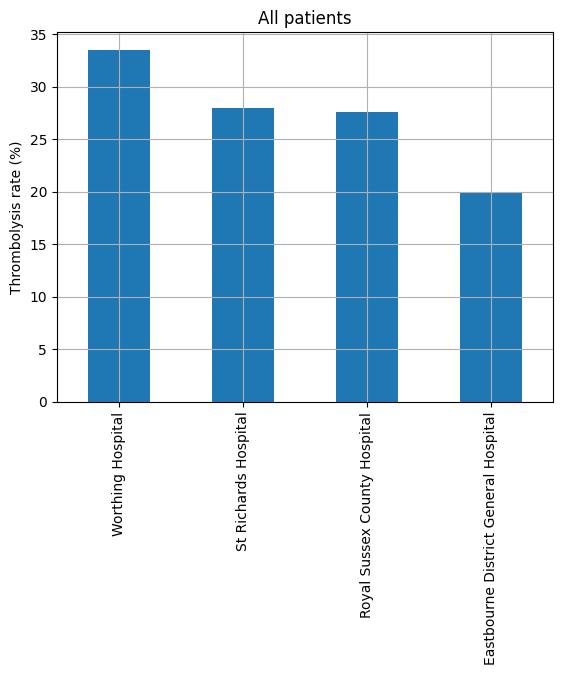
\includegraphics[width=1.0\textwidth]{./sussex/images/subgroup_all}
    \end{column}
    \begin{column}{0.5\textwidth}
      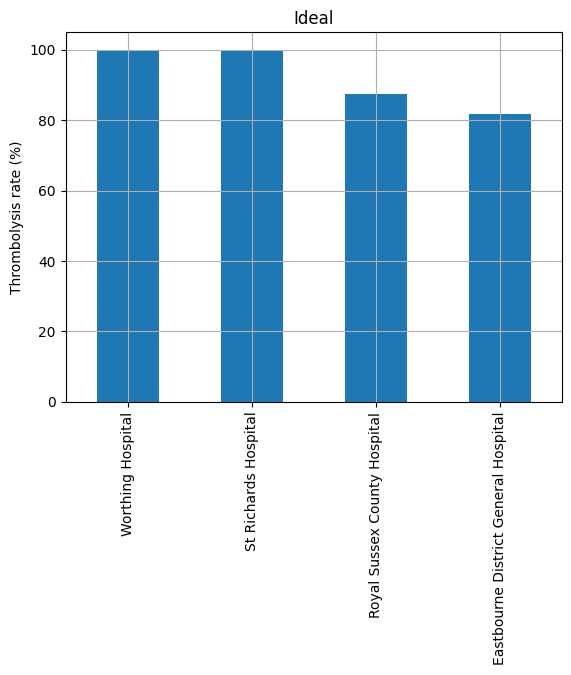
\includegraphics[width=1.0\textwidth]{./sussex/images/subgroup_ideal}
    \end{column}
  \end{columns}

\end{frame}

%%%%%%%%%%%%%%%%%%%%%%%%%%%%%%%%%%%%%%%%%%%%%%%%%%%%%%%%%%%%%%%%%%%%%%%%%%%%%%%%%

\begin{frame}
\frametitle{Observed thrombolysis use in subgroups (2)}

  \begin{columns}[T]
    \begin{column}{0.5\textwidth}
      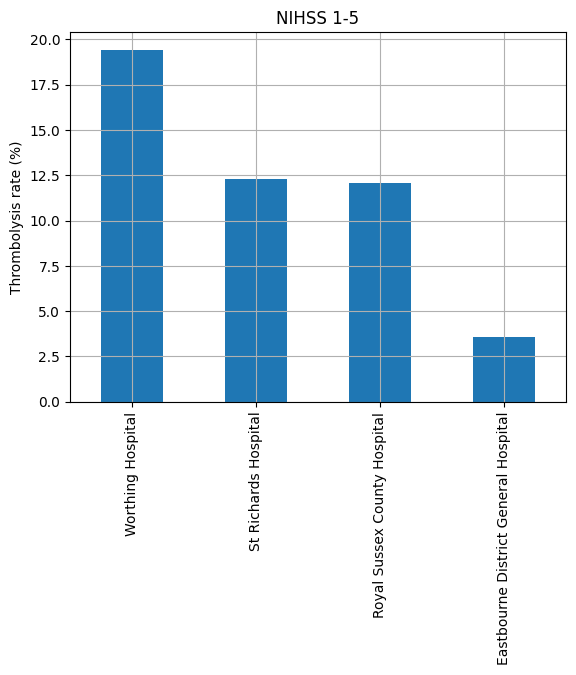
\includegraphics[width=1.0\textwidth]{./sussex/images/subgroup_mild}
    \end{column}
    \begin{column}{0.5\textwidth}
      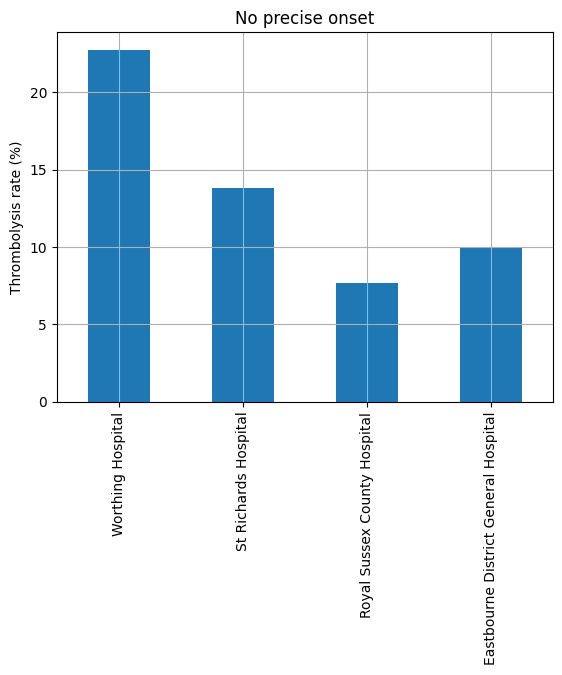
\includegraphics[width=1.0\textwidth]{./sussex/images/subgroup_precise}
    \end{column}
  \end{columns}

\end{frame}

%%%%%%%%%%%%%%%%%%%%%%%%%%%%%%%%%%%%%%%%%%%%%%%%%%%%%%%%%%%%%%%%%%%%%%%%%%%%%%%%%

\begin{frame}
\frametitle{Observed thrombolysis use in subgroups (3)}

  \begin{columns}[T]
    \begin{column}{0.5\textwidth}
      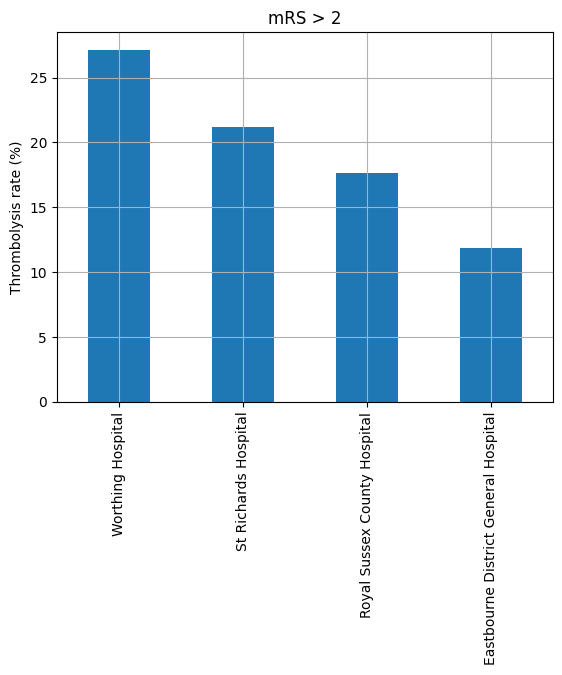
\includegraphics[width=1.0\textwidth]{./sussex/images/subgroup_disability}
    \end{column}
    \begin{column}{0.5\textwidth}
      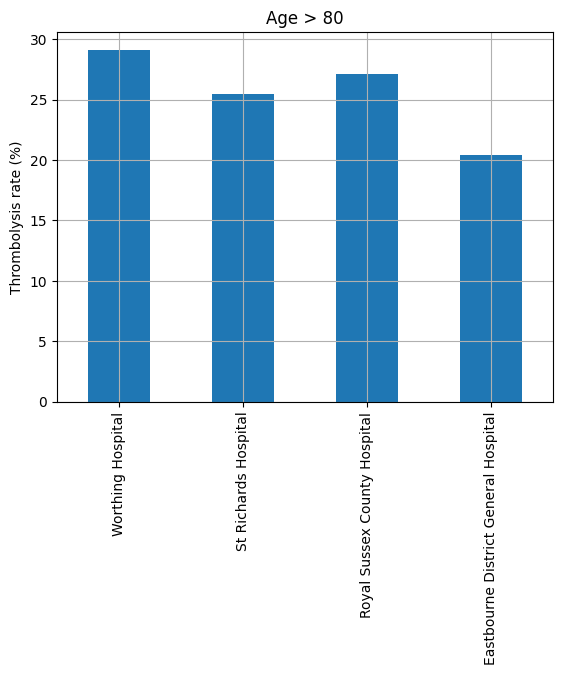
\includegraphics[width=1.0\textwidth]{./sussex/images/subgroup_age}
    \end{column}
  \end{columns}

\end{frame}



\begin{frame}
\frametitle{Predicted subgroup thrombolysis for 10k cohort}

As subgroup patient characteristics can vary between hopsitals, we also predict use of throbolysis in the same 10k cohort of patients at all hospitals.

\vspace{4mm}

\normalsize
\textbf{Observed thrombolysis:}
\scriptsize
\begin{table}[]
\begin{tabular}{rrrrrrr}
\textbf{}    & All (4hr) & Ideal & NIHSS 1-5 & No precise & mRS \textgreater 2 & Age \textgreater 80 \\
\hline
Worthing     & 33.5         & 100.0 & 19.4      & 22.8       & 27.2               & 29.1                \\
St Richards  & 28.0         & 100.0 & 12.3      & 13.8       & 21.2               & 25.5                \\
Royal Sussex & 27.6         & 87.5  & 12.0      & 7.7        & 17.6               & 27.1                \\
Eastbourne   & 20.0         & 81.8  & 3.6       & 9.9        & 11.9               & 20.4               
\end{tabular}
\end{table}

\vspace{2mm}
\normalsize
\textbf{Predicted average probability of thrombolysis in 10k cohort:}
\scriptsize
\begin{table}[]
\begin{tabular}{rrrrrrr}
\textbf{}    & All (4hr) & Ideal & NIHSS 1-5 & No precise & mRS \textgreater 2 & Age \textgreater 80 \\
\hline
Worthing     & 36.5         & 95.4  & 24.1      & 20.8             & 25.2               & 30.6                \\
St Richards  & 34.0         & 91.3  & 19.2      & 17.6             & 26.0               & 30.6                \\
Royal Sussex & 25.2         & 83.9  & 12.9      & 10.3             & 14.5               & 20.0                \\
Eastbourne  & 17.9         & 76.6  & 4.5       & 8.9              & 10.5               & 14.8               
\end{tabular}
\end{table}

\end{frame}


\begin{frame}
\frametitle{Benchmark thrombolysis decisions}


\begin{table}[]
\begin{tabular}{rrr}
                            & actual & benchmark \\
\hline
Worthing                    & 0.34   & 0.30      \\
St Richards                 & 0.28   & 0.29     \\
Royal Sussex County         & 0.28   & 0.43     \\
Eastbourne                  & 0.20   & 0.41
\end{tabular}
\end{table}

\end{frame}
\begin{frame}
\frametitle{Web application}

\begin{itemize}
    \item Introduction video: \url{https://youtu.be/V-uNbNK0XTc}
    \item Web app: \url{https://stroke-predictions.streamlit.app/Thrombolysis_decisions}
    \item Detailed work: \url{https://samuel-book.github.io/samuel_shap_paper_1/}
    \item Susses hospital codes in Webb App:
    \begin{itemize}
        \item Royal Sussex: 149
        \item Eastbourn: 151
        \item Worthing: 171
        \item St Richards: 177
    \end{itemize}
\end{itemize}

\vspace{3mm}
Note: Web App is experimental, and we may need to move to a higher performance server if multiple people access it the same time (which we don't think is very likely, but who knows?!).
 
\end{frame}

%%%%%%%%%%%%%%%%%%%%%%%%%%%%%%%%%%%%%%%%%%%%%%%%%%%%%%%%%%%%%%%


\end{document}
